% Chapter 1, Section 2 _Linear Algebra_ Jim Hefferon
%  http://joshua.smcvt.edu/linalg.html
%  2001-Jun-09
\section{Linear Geometry}
\textit{If you have seen the elements of vectors before then
this section is an optional review.
However, later work will refer to this material
so if this is not a review then it is not optional.}

In the first section, we had to do a bit of work to show
that there are only three types of solution sets\Dash singleton, empty, and
infinite.
But in the special case of systems with two equations and two unknowns
this is easy to see with a picture.
Draw each two-unknowns equation as a line in the plane and then
the two lines could have a unique intersection, 
be parallel, or be the same line.
%<*diagram:ThreeKindsSolutionSets>
\begin{center}
  \begin{minipage}[b]{1.45in}
    \raisebox{-2pt}[8pt][0pt]{\small \begin{tabular}{@{}l}
      \small \textit{Unique solution}
    \end{tabular}}
    \begin{center}
      \includegraphics{ch1.3} \\[.75ex]
      \small $\begin{linsys}{2}
                         3x  &+  &2y  &=  &7   \\
                         x   &-  &y   &=  &-1
                       \end{linsys}$
    \end{center}
  \end{minipage}
  \hspace*{0em}
  \begin{minipage}[b]{1.45in}
    \raisebox{-2pt}[8pt][0pt]{\small \begin{tabular}{@{}l}
      \small \textit{No solutions}
    \end{tabular}}
    \begin{center}
      \includegraphics{ch1.4} \\[.75ex]
      \small $\begin{linsys}{2}
                         3x  &+  &2y  &=  &7   \\
                         3x  &+  &2y  &=  &4
                       \end{linsys}$
    \end{center}
  \end{minipage}
  \hspace*{0em}
  \begin{minipage}[b]{1.45in}
    \raisebox{-2pt}[8pt][0pt]{\small \begin{tabular}[t]{@{}l}
      \textit{Infinitely many} \\
      \textit{solutions}
    \end{tabular}}
    \begin{center}
      \includegraphics{ch1.5}         \\[.75ex]
      \small $ \begin{linsys}{2}
                         3x  &+  &2y  &=  &7   \\
                         6x  &+  &4y  &=  &14
                       \end{linsys}$
    \end{center}
  \end{minipage}
\end{center}
%</diagram:ThreeKindsSolutionSets>
These pictures aren't a short way to prove
the results from the prior section, because those apply
to any number of linear equations and any number of unknowns. 
But they do help us understand those results.
This section develops the ideas that we need to
express our results geometrically. 
In particular, while
the two-dimensional case is familiar, to extend to systems with
more than two unknowns we shall need some higher-dimensional geometry.














\subsectionoptional{Vectors in Space}
``Higher-dimensional geometry'' sounds exotic.
It is exotic\Dash interesting and eye-opening.
But it isn't distant or unreachable.

We begin by defining one-dimensional space to be \( \Re^1 \).
To see that the definition is reasonable, 
we picture a one-dimensional space
\begin{center}
  \includegraphics{ch1.6}
\end{center}
and make a correspondence with \( \Re \) by
picking a point to label $0$ and another to label $1$.
\begin{center}
  \includegraphics{ch1.7}
\end{center}
Now, with a scale and a direction,
finding the point corresponding to, say,
\( +2.17 \), is easy\Dash start at \( 0 \) and head in the direction of \( 1 \),
but don't stop there, go \( 2.17 \) times as far.

The basic idea here, combining magnitude with direction, is the
key to extending to higher dimensions.

An object comprised of a magnitude and a direction is a
\definend{vector\/}\index{vector}
(we use the same word as in the prior section because we shall show
below how to describe such
an object with a column vector).
We can draw a vector as having some length, and pointing somewhere.
\begin{center}
  \includegraphics{ch1.8}
\end{center}
There is a subtlety here\Dash these vectors
\begin{center}
  \includegraphics{ch1.9}
\end{center}
are equal, even though they start in different places,
because they have equal lengths and equal directions.
Again: those vectors are not just alike, they are equal.

How can things that are in different places be equal?
Think of a vector as representing a displacement
(the word vector is Latin for ``carrier'' or ``traveler'').
These two squares undergo equal displacements,
despite that those displacements start in different places. 
\begin{center}
  \includegraphics{ch1.10}
\end{center}
Sometimes, to emphasize this property vectors have of not being anchored,
we can refer to them as \definend{free}\index{vector!free} vectors.
Thus, these free vectors are equal
as each is a displacement of one over and two up.
\begin{center}
  \includegraphics{ch1.12}
\end{center}
More generally, vectors in the plane 
are the same if and only if they have the same
change in first components and the same change in second components:~the
vector extending from \( (a_1,a_2) \)
to \( (b_1,b_2) \) equals the vector from 
\( (c_1,c_2) \) to \( (d_1,d_2) \)
if and only if 
\( b_1-a_1=d_1-c_1 \) and \( b_2-a_2=d_2-c_2 \).

Saying `the vector that, were it to start at \( (a_1,a_2) \),
would extend to \( (b_1,b_2) \)' would be unwieldy.
We instead describe that vector as
\begin{equation*}
  \colvec{b_1-a_1 \\ b_2-a_2}
\end{equation*}
so that the `one over and two up' arrows shown above 
picture this vector.
\begin{equation*}
  \colvec[r]{1 \\ 2}
\end{equation*}
We often draw the arrow as starting at the origin, and we
then say it is in the 
\definend{canonical position}\index{vector!canonical position}
(or \definend{natural position}\index{vector!natural position} 
or \definend{standard position}\index{vector!standard position}). 
When the vector
\begin{equation*}
  \colvec{v_1 \\ v_2}
\end{equation*}
is in canonical position then it
extends to the endpoint $(v_1,v_2)$.

We typically just refer to ``the point
\begin{equation*}
  \colvec[r]{1 \\ 2}\text{''}
\end{equation*}
rather than ``the endpoint of the canonical position of'' that vector.
% That is, we shall find it convienent to blur the distinction between a point
% in space and the vector that, if it starts at the origin, ends at that 
% point.
Thus, we will call each of these \( \Re^2 \).
\begin{equation*}
   \set{(x_1,x_2)\suchthat x_1,x_2\in\Re}
   \qquad
   \set{\colvec{x_1 \\ x_2}\suchthat x_1,x_2\in\Re}
\end{equation*}

In the prior section we defined vectors and vector operations
with an algebraic motivation;
\begin{equation*}
   r\cdot\colvec{v_1 \\ v_2}
   =
   \colvec{rv_1 \\ rv_2}
  \qquad
   \colvec{v_1 \\  v_2}
   +
   \colvec{w_1 \\ w_2}
   =
   \colvec{v_1+w_1 \\ v_2+w_2}
\end{equation*}
we can now understand those operations geometrically.
\index{vector!sum}\index{vector!scalar multiple}\index{sum!vector}
\index{scalar multiple!vector}
For instance, if \( \vec{v} \) represents a displacement
then \( 3\vec{v}\, \) represents a displacement in the same direction but 
three times as far,
and \( -1\vec{v}\, \) represents a displacement of the same distance as
\( \vec{v}\, \) but in the opposite direction.
\begin{center}
  \includegraphics{ch1.13}
\end{center}
And, where \( \vec{v} \) and \( \vec{w} \) represent displacements,
\( \vec{v}+\vec{w}\/ \) represents those displacements combined.
\begin{center}
  \includegraphics{ch1.14}
\end{center}
The long arrow is the combined displacement in this sense:~if, in one minute, 
a ship's motion gives it the displacement 
relative to the earth of $\vec{v}$ and a passenger's
motion gives a displacement relative to the ship's deck of $\vec{w}$,
then $\vec{v}+\vec{w}\/$ is the
displacement of the passenger relative to the earth.

Another way to understand the vector sum is with the
\definend{parallelogram rule}.\index{parallelogram rule}%
\index{vector!sum}
Draw the parallelogram 
formed by the vectors $\vec{v}$ and $\vec{w}$.
Then the sum $\vec{v}+\vec{w}$ extends along the diagonal 
to the far corner.
\begin{center}
  \includegraphics{ch1.15}
\end{center}

The above drawings show how vectors and vector operations
behave in \( \Re^2 \).
We can extend to $\Re^3$, or to even higher-dimensional spaces
where we have no pictures, with the obvious generalization:~the 
free vector that, 
if it starts at \( (a_1,\ldots,a_n) \), ends at \( (b_1,\ldots,b_n) \), 
is represented by this column.
\begin{equation*}
  \colvec{b_1-a_1 \\ \vdotswithin{b_1-a_1} \\ b_n-a_n}
\end{equation*}
Vectors are equal if they have the same representation.
We aren't too careful about distinguishing between a point and the vector whose
canonical representation ends at that point. 
\begin{equation*}
  \Re^n=
  \set{\colvec{v_1 \\ \vdotswithin{v_1} \\ v_n}\suchthat v_1,\ldots,v_n\in\Re}
\end{equation*}
And, we do addition and scalar multiplication component-wise.

Having considered points, we now turn to the lines.
In $\Re^2$, the line through \( (1,2) \) and \( (3,1) \)
is comprised of (the endpoints of) the vectors in this set.
\begin{equation*}
   \set{ \colvec[r]{1 \\ 2}+t\colvec[r]{2 \\ -1}\suchthat t\in\Re}
\end{equation*}
That description expresses this picture.
\begin{center}
  \includegraphics{ch1.16}
\end{center}
The vector associated with the parameter \( t \)
\begin{equation*}
  \colvec[r]{2 \\ -1}=\colvec[r]{3 \\ 1}-\colvec[r]{1 \\ 2}
\end{equation*}
has its whole body in the line\Dash it
is a \definend{direction vector}\index{vector!direction}%
\index{direction vector} for the line.
Note that points on the line to the left of \( x=1 \) are described
using negative values of \( t \).
% Note also that this description of lines generalizes the familiar 
% $y=b+mx$ form for lines in the plane.

In \( \Re^3 \),
the line through \( (1,2,1) \) and \( (2,3,2) \) is the set of
(endpoints of) vectors of this form
\begin{center}
  \includegraphics{ch1.17}
\end{center}
and lines in even higher-dimensional spaces work in the same way.

In $\Re^3$, 
a line uses one parameter so that a particle on that line  
is free to move back and forth 
in one dimension,
and a plane involves two parameters.
For example, the plane through the points
\( (1,0,5) \), \( (2,1,-3) \), and \( (-2,4,0.5) \) consists of
(endpoints of) the vectors in
\begin{equation*}
  \set{ \colvec[r]{1 \\ 0 \\ 5}
         +t\colvec[r]{1 \\ 1 \\ -8}
         +s\colvec[r]{-3 \\ 4 \\ -4.5}
       \suchthat t,s\in\Re      }
\end{equation*}
(the column vectors associated with the parameters
\begin{equation*}
  \colvec[r]{1 \\ 1 \\ -8}
  =
  \colvec[r]{2 \\ 1 \\ -3}
  -
  \colvec[r]{1 \\ 0 \\ 5}
  \qquad
  \colvec[r]{-3 \\ 4 \\ -4.5}
  =
  \colvec[r]{-2 \\ 4 \\ 0.5}
  -
  \colvec[r]{1 \\ 0 \\ 5}
\end{equation*}
are two vectors whose whole bodies lie in the plane).
As with the line, note that we describe some points in this plane
with negative $t$'s or negative $s$'s or both.

In algebra and calculus we often use a description of planes involving 
a single equation
as the condition that describes 
the relationship among the first, second, and third
coordinates of points in a plane.
% \newsavebox{\jhscratchbox}
% \savebox{\jhscratchbox}{\includegraphics{ch1.18}}
% \newlength{\jhscratchlength}\newlength{\jhscratchheight}
% \settowidth{\jhscratchlength}{\usebox{\jhscratchbox}}
\begin{equation*}
  % \usebox{\jhscratchbox}
  \vcenteredhbox{\includegraphics{ch1.18}}
\end{equation*}
% \begin{equation*}
%   P=\set{\colvec{x \\ y \\ z}\suchthat 2x+3y-z=4}
% \end{equation*}
The translation from such a description to the vector description that we
favor in this book is to 
think of the condition as a one-equation linear system
and parametrize \( x=2-y/2-z/2 \).
\begin{equation*}
   \vcenteredhbox{\includegraphics{ch1.19}}
\end{equation*}
% \begin{center}
%   \makebox[\jhscratchlength][l]{\includegraphics{ch1.20}}
% \end{center}
% \begin{equation*}
%   P=\set{\colvec[r]{2 \\ 0 \\ 0}
%          +y\cdot\colvec[r]{-1/2 \\ 1 \\ 0}
%          +z\cdot\colvec[r]{-1/2 \\ 0 \\ 1}\suchthat y,z\in\Re}
% \end{equation*}
Generalizing, a set of the form
$\set{\vec{p}+t_1\vec{v}_1+t_2\vec{v}_2+\cdots+t_k\vec{v}_k
             \suchthat t_1,\ldots ,t_k\in\Re}$
where \( \vec{v}_1,\ldots,\vec{v}_k\in\Re^n \) 
and $k\leq n$ is a
\definend{\( k \)-dimensional linear surface}\index{linear surface}
(or \definend{\( k \)-flat}\index{flat}). 
For example, in $\Re^4$
\begin{equation*}
  \set{\colvec[r]{2 \\ \pi \\ 3 \\ -0.5}
       +t\colvec[r]{1 \\ 0 \\ 0 \\ 0}
       \suchthat t\in\Re}
\end{equation*}
is a line,
\begin{equation*}
  \set{
       \colvec[r]{0 \\ 0 \\ 0 \\ 0}
       +t\colvec[r]{1 \\ 1 \\ 0 \\ -1}
       +s\colvec[r]{2 \\ 0 \\ 1 \\ 0}
       \suchthat t,s\in\Re}
\end{equation*}
is a plane, and
\begin{equation*}
  \set{
       \colvec[r]{3 \\ 1 \\ -2 \\ 0.5}
       +r\colvec[r]{0 \\ 0 \\ 0 \\ -1}
       +s\colvec[r]{1 \\ 0 \\ 1 \\ 0}
       +t\colvec[r]{2 \\ 0 \\ 1 \\ 0}
       \suchthat r,s,t\in\Re}
\end{equation*}
is a three-dimensional linear surface.
Again, the intuition is that a line permits motion in one direction,
a plane permits motion in
combinations of two directions, etc.
(When the dimension of the linear surface is one less than the dimension 
of the space, that is, when we have an 
$n-1$-flat in $\Re^n$, 
then the surface is called a 
\definend{hyperplane}.\index{hyperplane})

A description of 
a linear surface can be misleading about the dimension.
For example, this
\begin{equation*}
  L=\set{
       \colvec[r]{1 \\ 0 \\ -1 \\ -2}
       +t\colvec[r]{1 \\ 1 \\ 0 \\ -1}
       +s\colvec[r]{2 \\ 2 \\ 0 \\ -2}
       \suchthat t,s\in\Re}
\end{equation*}
is a \definend{degenerate} plane because it is actually a line,
since the
vectors are multiples of each other so we
can merge the two into one.
\begin{equation*}
  L=\set{
       \colvec[r]{1 \\ 0 \\ -1 \\ -2}
       +r\colvec[r]{1 \\ 1 \\ 0 \\ -1}
       \suchthat r\in\Re}
\end{equation*}
We shall see in the Linear Independence section of Chapter Two
what relationships among vectors causes the linear surface
they generate to be degenerate.

We finish this subsection
by restating our conclusions from earlier in geometric terms.
First, the solution set of a linear system with \( n \) unknowns
is a linear surface in \( \Re^n \).
Specifically, it is a \( k \)-dimensional linear surface, where
\( k \) is the number of free variables in an echelon form version 
of the system.
Second, the solution set of a homogeneous linear system is a linear surface
passing through the origin.
Finally, we can view the general solution set of any
linear system as being the solution set of its associated homogeneous system
offset from the origin by a vector,
namely by any particular solution.




\begin{exercises}
  \recommended \item
    Find the canonical name for each vector.
    \begin{exparts}
      \partsitem the vector from \( (2,1) \) to \( (4,2) \) in \( \Re^2 \)
      \partsitem the vector from \( (3,3) \) to \( (2,5) \) in \( \Re^2 \)
      \partsitem the vector from \( (1,0,6) \) to \( (5,0,3) \) in \( \Re^3 \)
      \partsitem the vector from \( (6,8,8) \) to \( (6,8,8) \) in \( \Re^3 \)
    \end{exparts}
    \begin{answer}
      \begin{exparts*}
        \partsitem \( \colvec[r]{2 \\ 1}  \)
        \partsitem \( \colvec[r]{-1 \\ 2}  \)
        \partsitem \( \colvec[r]{4 \\ 0 \\ -3}  \)
        \partsitem \( \colvec[r]{0 \\ 0 \\ 0}  \)
      \end{exparts*}  
     \end{answer}
  \recommended \item 
    Decide if the two vectors are equal.
    \begin{exparts}
      \partsitem the vector from \( (5,3) \) to \( (6,2) \) and the vector
        from \( (1,-2) \) to \( (1,1) \)
      \partsitem the vector from \( (2,1,1) \) to \( (3,0,4) \) and the vector
        from \( (5,1,4) \) to \( (6,0,7) \)
    \end{exparts}
    \begin{answer}
      \begin{exparts}
        \partsitem No, their canonical positions are different.
          \begin{equation*}
            \colvec[r]{1 \\ -1}
            \qquad
            \colvec[r]{0 \\ 3}
          \end{equation*}
        \partsitem Yes, their canonical positions are the same.
          \begin{equation*}
            \colvec[r]{1 \\ -1 \\ 3}
          \end{equation*}
      \end{exparts}  
     \end{answer}
  \recommended \item
    Does \( (1,0,2,1) \) lie on the line through
    \( (-2,1,1,0) \) and \( (5,10,-1,4) \)?
    \begin{answer}
      That line is this set.
      \begin{equation*}
        \set{\colvec[r]{-2 \\ 1 \\ 1 \\ 0}
             +\colvec[r]{7 \\ 9 \\ -2 \\ 4}t \suchthat t\in\Re }
      \end{equation*}
      Note that this system
      \begin{equation*}
        \begin{linsys}{2}
          -2  &+  &7t  &=  &1  \\
           1  &+  &9t  &=  &0  \\
           1  &-  &2t  &=  &2  \\
           0  &+  &4t  &=  &1  
        \end{linsys}
      \end{equation*}
      has no solution.
      Thus the given point is not in the line.  
    \end{answer}
  \recommended \item
     \begin{exparts}
        \partsitem Describe the plane through \( (1,1,5,-1) \),
           \( (2,2,2,0) \), and \( (3,1,0,4) \).
        \partsitem Is the origin in that plane?
      \end{exparts}
    \begin{answer}
      \begin{exparts}
        \partsitem Note that
          \begin{equation*}
            \colvec[r]{2 \\ 2 \\ 2 \\ 0}
            -\colvec[r]{1 \\ 1 \\ 5 \\ -1}
            =\colvec[r]{1 \\ 1 \\ -3 \\ 1}
            \qquad
            \colvec[r]{3 \\ 1 \\ 0 \\ 4}
            -\colvec[r]{1 \\ 1 \\ 5 \\ -1}
            =\colvec[r]{2 \\ 0 \\ -5 \\ 5}
          \end{equation*}
          and so the plane is this set.
          \begin{equation*}
            \set{\colvec[r]{1 \\ 1 \\ 5 \\ -1}
                 +\colvec[r]{1 \\ 1 \\ -3 \\ 1}t
                 +\colvec[r]{2 \\ 0 \\ -5 \\ 5}s
                \suchthat t,s\in\Re}
          \end{equation*}
        \partsitem No; this system
          \begin{equation*}
            \begin{linsys}{3}
              1  &+  &1t  &+  &2s  &=  &0  \\
              1  &+  &1t  &   &    &=  &0  \\
              5  &-  &3t  &-  &5s  &=  &0  \\
             -1  &+  &1t  &+  &5s  &=  &0  
            \end{linsys}
          \end{equation*}
          has no solution.
      \end{exparts}  
    \end{answer}
  \item 
    Describe the plane that contains this point and line.
    \begin{equation*}
      \colvec[r]{2 \\ 0 \\ 3}
      \qquad
      \set{\colvec[r]{-1 \\ 0 \\ -4}
           +\colvec[r]{1 \\ 1 \\ 2}t
           \suchthat t\in\Re}
    \end{equation*}
    \begin{answer}
      The vector
      \begin{equation*}
        \colvec[r]{2 \\ 0 \\ 3}
      \end{equation*}
      is not in the line.
      Because
      \begin{equation*}
        \colvec[r]{2 \\ 0 \\ 3}
        -\colvec[r]{-1 \\ 0 \\ -4}
        =\colvec[r]{3 \\ 0 \\ 7}
      \end{equation*}
      we can describe that plane in this way.
      \begin{equation*}
        \set{\colvec[r]{-1 \\ 0 \\ -4}
             +m\colvec[r]{1 \\ 1 \\ 2}
             +n\colvec[r]{3 \\ 0 \\ 7}
            \suchthat m,n\in\Re}
      \end{equation*}  
   \end{answer}
  \recommended \item
    Intersect these planes.
    \begin{equation*}
      \set{\colvec[r]{1 \\ 1 \\ 1}t+
           \colvec[r]{0 \\ 1 \\ 3}s
           \suchthat t,s\in\Re}
      \qquad
      \set{\colvec[r]{1 \\ 1 \\ 0}
           +\colvec[r]{0 \\ 3 \\ 0}k+
           \colvec[r]{2 \\ 0 \\ 4}m
           \suchthat k,m\in\Re}
    \end{equation*}
    \begin{answer}
      The points of coincidence are solutions of this system.
      \begin{equation*}
        \begin{linsys}{2}
         t  &  &   &= &1+2m\hfill      \\
         t  &+ &s  &= &1+3k\hfill      \\
         t  &+ &3s &= &4m\hfill
        \end{linsys}
      \end{equation*}
      Gauss's Method
      \begin{equation*}
        \begin{amat}{4}
          1  &0  &0  &-2  &1  \\
          1  &1  &-3 &0   &1  \\
          1  &3  &0  &-4  &0
        \end{amat}
        \;\grstep[-\rho_1+\rho_3]{-\rho_1+\rho_2}\;
        \begin{amat}{4}
          1  &0  &0  &-2  &1  \\
          0  &1  &-3 &2   &0  \\
          0  &3  &0  &-2  &-1
        \end{amat}                         
        \;\grstep{-3\rho_2+\rho_3}\;
        \begin{amat}{4}
          1  &0  &0  &-2  &1  \\
          0  &1  &-3 &2   &0  \\
          0  &0  &9  &-8  &-1
        \end{amat}
      \end{equation*}
      gives \( k=-(1/9)+(8/9)m \), so \( s=-(1/3)+(2/3)m \) and \( t=1+2m \).
      The intersection is this.
      \begin{equation*}
        \set{\colvec[r]{1 \\ 1 \\ 0}+
             \colvec[r]{0 \\ 3 \\ 0}(-\frac{1}{9}+\frac{8}{9}m)+
             \colvec[r]{2 \\ 0 \\ 4}m
             \suchthat m\in\Re}
        =\set{\colvec[r]{1 \\ 2/3 \\ 0}
             +\colvec[r]{2 \\ 8/3 \\ 4}m
             \suchthat m\in\Re}
      \end{equation*}    
    \end{answer}
  \recommended \item
    Intersect each pair, if possible.
    \begin{exparts}
      \partsitem \( \set{\colvec[r]{1 \\ 1 \\ 2}+t\colvec[r]{0 \\ 1 \\ 1}
                     \suchthat t\in\Re} \),
            \( \set{\colvec[r]{1 \\ 3 \\ -2}+s\colvec[r]{0 \\ 1 \\ 2}
                     \suchthat s\in\Re} \)
      \partsitem \( \set{\colvec[r]{2 \\ 0 \\ 1}+t\colvec[r]{1 \\ 1 \\ -1}
                     \suchthat t\in\Re} \),
            \( \set{s\colvec[r]{0 \\ 1 \\ 2}
                     +w\colvec[r]{0 \\ 4 \\ 1}
                     \suchthat s,w\in\Re} \)
    \end{exparts}
    \begin{answer}
       \begin{exparts}
        \partsitem The system
          \begin{equation*}
            \begin{linsys}{1}
              1     &= &1\hfill         \\
              1+t   &= &3+s\hfill         \\
              2+t   &= &-2+2s\hfill
            \end{linsys}
          \end{equation*}
          gives \( s=6 \) and \( t=8 \), so this is the solution set.
          \begin{equation*}
            \set{\colvec[r]{1 \\ 9 \\ 10}     }
          \end{equation*}
        \partsitem This system
          \begin{equation*}
            \begin{linsys}{1}
            2+t   &=  &0 \hfill        \\
            t     &=  &s+4w\hfill        \\
            1-t   &=  &2s+w\hfill
            \end{linsys}
          \end{equation*}
          gives \( t=-2 \), \( w=-1 \), and \( s=2 \) so their intersection
          is this point.
          \begin{equation*}
            \colvec[r]{0 \\ -2 \\ 3}
          \end{equation*}
      \end{exparts}  
    \end{answer}
  \item 
    When a plane does not pass through the origin, performing
    operations on vectors whose bodies lie in it
    is more complicated than when
    the plane passes through the origin.
    Consider the picture in this subsection of the plane 
    \begin{equation*}
      \set{\colvec[r]{2 \\ 0 \\ 0}
            +\colvec[r]{-0.5 \\ 1 \\ 0} y
            +\colvec[r]{-0.5 \\ 0 \\ 1} z
            \suchthat y,z\in\Re}
    \end{equation*}
    and the three vectors with endpoints
    $(2,0,0)$, $(1.5,1,0)$, and $(1.5,0,1)$.
    \begin{exparts}
      \partsitem Redraw the picture, including the vector 
        in the plane that is twice as long as the one with
        endpoint $(1.5,1,0)$.
        The endpoint of your vector is not $(3,2,0)$; what is it?
      \partsitem Redraw the picture, including the parallelogram 
        in the plane that shows the sum of the vectors 
        ending at $(1.5,0,1)$ and $(1.5,1,0)$.
        The endpoint of the sum, on the diagonal, is not $(3,1,1)$; what is it?
    \end{exparts}
    \begin{answer}
      \begin{exparts}
        \partsitem The vector shown
          \begin{center}
            \includegraphics{ch1.32}
          \end{center}
          is not the result of doubling
          \begin{equation*}
            \colvec[r]{2 \\ 0 \\ 0}
              +\colvec[r]{-0.5 \\ 1 \\ 0}\cdot 1
          \end{equation*}
          instead it is 
          \begin{equation*}
            \colvec[r]{2 \\ 0 \\ 0}
              +\colvec[r]{-0.5 \\ 1 \\ 0}\cdot 2
            =\colvec[r]{1 \\ 2 \\ 0}
          \end{equation*}
          which has a parameter twice as large.
        \partsitem The vector
          \begin{center}
            \includegraphics{ch1.19}
          \end{center}
          is not the result of adding
          \begin{equation*}
            (\colvec[r]{2 \\ 0 \\ 0}
              +\colvec[r]{-0.5 \\ 1 \\ 0}\cdot 1)
            +
            (\colvec[r]{2 \\ 0 \\ 0}
              +\colvec[r]{-0.5 \\ 0 \\ 1}\cdot 1)
          \end{equation*}
          instead it is 
          \begin{equation*}
            \colvec[r]{2 \\ 0 \\ 0}
              +\colvec[r]{-0.5 \\ 1 \\ 0}\cdot 1
              +\colvec[r]{-0.5 \\ 0 \\ 1}\cdot 1
            =\colvec[r]{1 \\ 1 \\ 1}
          \end{equation*}
          which adds the parameters.
      \end{exparts}
    \end{answer}
  \item 
    Show that the line segments
    \( \overline{(a_1,a_2)(b_1,b_2)} \) and
    \( \overline{(c_1,c_2)(d_1,d_2)} \)
    have the same lengths and slopes if
    \(  b_1-a_1=d_1-c_1 \) and \( b_2-a_2=d_2-c_2 \).
    Is that only if?
    \begin{answer}
      The ``if'' half is straightforward.
      If \( b_1-a_1=d_1-c_1 \) and \( b_2-a_2=d_2-c_2 \) then
      \begin{equation*}
        \sqrt{(b_1-a_1)^2+(b_2-a_2)^2}
        =\sqrt{(d_1-c_1)^2+(d_2-c_2)^2}
      \end{equation*}
      so they have the same lengths, and the slopes are just as easy:
      \begin{equation*}
        \frac{b_2-a_2}{b_1-a_1}
        =\frac{d_2-c_2}{d_1-a_1}
      \end{equation*}
      (if the denominators are \( 0 \) they both have undefined slopes).

     For ``only if'', assume that
     the two segments have the same length and slope
     (the case of undefined slopes is easy; we will do the case where both
     segments have a slope \( m \)).
     Also assume, without loss of generality, that $a_1<b_1$ and that
     $c_1<d_1$.
     The first segment is
     \( \overline{(a_1,a_2)(b_1,b_2)}=
     \set{(x,y)\suchthat y=mx+n_1,\; x\in [a_1..b_1]} \)
     (for some intercept $n_1$)
     and the second segment is \( \overline{(c_1,c_2)(d_1,d_2)}=
     \set{(x,y)\suchthat y=mx+n_2,\; x\in [c_1..d_1]} \)
     (for some $n_2$).
     Then the lengths of those segments are
     \begin{equation*}
     \sqrt{(b_1-a_1)^2+((mb_1+n_1)-(ma_1+n_1))^2}
       =\sqrt{(1+m^2)(b_1-a_1)^2}
     \end{equation*}
     and, similarly, \( \sqrt{(1+m^2)(d_1-c_1)^2} \).
     Therefore, \( \absval{b_1-a_1}=\absval{d_1-c_1} \).
     Thus, as we assumed that \( a_1<b_1 \) and \( c_1<d_1 \), we have
     that \( b_1-a_1=d_1-c_1 \).

     The other equality is similar.   
   \end{answer}
  \item 
      How should we define $\Re^0$?
      \begin{answer}
        We shall later define it to be a set with one element\Dash an
        ``origin''.  
      \end{answer}
  \puzzle \recommended \item   
    \cite{MathMag57p173}
    A person traveling eastward at a rate of
    \( 3 \) miles per hour finds that the wind appears to blow directly
    from the north.
    On doubling his speed it appears to come from the north east.
    What was the wind's velocity?
    \begin{answer}
      \answerasgiven %
      The vector triangle is as follows, so \( \vec{w}=3\sqrt{2} \)
      from the north west.
      \begin{center}
        \setlength{\unitlength}{4pt}      % wind triangles.
        \begin{picture}(20,12)(0,0)
           \put(0,10){\vector(1,0){20} }
           \put(0,10){\vector(1,-1){10} }
              \put(3.8,5){\makebox(0,0)[r]{\small \( \vec{w} \)} }
           \put(10,0){\vector(1,1){10} }
           \put(10,0){\line(0,1){10} }
        \end{picture}
      \end{center}  
     \end{answer}
  \item \checked \label{exer:Euclid}  
    Euclid describes a plane as
    ``a surface which lies evenly with the straight lines on itself''.
    Commentators such as Heron have interpreted this to mean,
    ``(A plane surface is) such that, if a straight line pass through 
    two points
    on it, the line coincides wholly with it at every spot, all ways''.
    (Translations from \cite{Heath}, pp. 171-172.)
    Do planes, as described in this section, have that property?
    Does this description adequately define planes?
    \begin{answer}
      Euclid no doubt is picturing a plane inside of \( \Re^3 \).
      Observe, however, that both \( \Re^1 \) and \( \Re^2 \) also satisfy
      that definition.  
    \end{answer}
\end{exercises}
















\subsectionoptional{Length and Angle Measures}
We've translated the first section's results about solution sets into
geometric terms, to better understand those sets.
But we must be careful not to be misled by our own terms\Dash 
labeling subsets of
\( \Re^k \) of the forms
\( \set{\vec{p}+t\vec{v}\suchthat t\in\Re} \) and
\( \set{\vec{p}+t\vec{v}+s\vec{w}\suchthat t,s\in\Re} \)
as `lines' and `planes' doesn't make them act like the lines
and planes of our past experience.
Rather, we must ensure that the names suit the sets.
While we can't prove that the sets satisfy our intuition\Dash we can't
prove anything about intuition\Dash in this subsection we'll observe that
a result familiar from \( \Re^2 \) and \( \Re^3 \), when generalized to
arbitrary \( \Re^n \), supports the idea that a line is straight
and a plane is flat.
Specifically, we'll see how to do Euclidean geometry in a ``plane'' by giving
a definition of the angle between two $\Re^n$ vectors in the plane that they
generate.

\begin{definition} \label{df:Length}
%<*df:Length>
The \definend{length}\index{vector!length}\index{length} 
(or \definend{norm}\index{vector!norm}\index{norm})
of a vector
\( \vec{v}\in\Re^n \) is the square root of the sum of the squares of its 
components.
\begin{equation*}
  \norm{\vec{v}\,}=\sqrt{v_1^2+\cdots+v_n^2}
\end{equation*}
%</df:Length>
\end{definition}

\begin{remark}
This is a natural generalization of the Pythagorean Theorem.
A classic discussion is in \cite{MathematicsPlausReason}.
\end{remark}

Note that for any nonzero $\vec{v}$, the vector $\vec{v}/\norm{\vec{v}}$
has length one.
We say that the second vector 
\definend{normalizes}\index{normalize}\index{vector!normalize}
$\vec{v}$ to length one. 

We can use that to get a formula 
for the angle between two vectors.
Consider two vectors in \( \Re^3 \)
where neither is a multiple of the other
\begin{center}
  \includegraphics{ch1.21}
\end{center}
(the special case of multiples will prove below not to be an exception).
They determine a two-dimensional plane\Dash
for instance, put them in canonical poistion and take the plane formed
by the origin and the endpoints.
In that plane consider the triangle with sides
\( \vec{u} \), \( \vec{v} \), and \( \vec{u}-\vec{v} \).
\begin{center}
  \includegraphics{ch1.22}
\end{center}
Apply the Law of Cosines:
$\norm{\vec{u}-\vec{v}\,}^2
  =
  \norm{\vec{u}\,}^2+\norm{\vec{v}\,}^2-
    2\,\norm{\vec{u}\,}\,\norm{\vec{v}\,}\cos\theta$ 
where \( \theta \) is the angle between the vectors.
The left side gives 
\begin{multline*}
(u_1-v_1)^2+(u_2-v_2)^2+(u_3-v_3)^2  \\
     =(u_1^2-2u_1v_1+v_1^2)+(u_2^2-2u_2v_2+v_2^2)+(u_3^2-2u_3v_3+v_3^2)
\end{multline*}
while the right side gives this.
\begin{equation*}
(u_1^2+u_2^2+u_3^2)+(v_1^2+v_2^2+v_3^2)-
     2\,\norm{\vec{u}\,}\,\norm{\vec{v}\,}\cos\theta
\end{equation*}
Canceling squares $u_1^2$, \ldots, $v_3^2$ and dividing by $2$ gives 
the formula.
\begin{equation*}
  \theta
  =
  \arccos(\,\frac{u_1v_1+u_2v_2+u_3v_3}{
         \norm{\vec{u}\,}\,\norm{\vec{v}\,} }\,)
\end{equation*}

To give a definition of angle that works in higher dimensions 
we cannot draw pictures but
we can make the argument analytically.

First, the form of the numerator is clear\Dash it comes from the middle terms
of \( (u_i-v_i)^2 \).

\begin{definition} \label{df:DotProduct}
%<*df:DotProduct>
The \definend{dot product}\index{vector!dot product}\index{dot product}
(or \definend{inner product}\index{inner product}
or \definend{scalar product}\index{scalar product})
of two \( n \)-component 
real vectors is the linear combination of their components.
\begin{equation*}
  \vec{u}\dotprod\vec{v}=\lincombo{u}{v}
\end{equation*}
%</df:DotProduct>
\end{definition}
Note that the dot product of two vectors is a real number, not a vector, and
that the dot product of a vector from \( \Re^n \) with a vector
from \( \Re^m \) is not defined unless \( n \) equals \( m \).
Note also this relationship between dot product and length:
\( \vec{u}\dotprod\vec{u}=u_1u_1+\cdots+u_nu_n=\norm{\vec{u}\,}^2 \). 

\begin{remark}
Some authors require that the first vector be a row vector and that the 
second vector be a column vector.
We shall not be that strict and will allow the dot product operation between
two column vectors.
\end{remark}

Still reasoning with letters but guided by the pictures,
we use the next theorem to argue that the triangle formed by
\( \vec{u} \), \( \vec{v} \), and \( \vec{u}-\vec{v} \) in \( \Re^n \)
lies in the planar subset of \( \Re^n \) generated by \( \vec{u} \) and
\( \vec{v} \).

\begin{theorem}[Triangle Inequality] \label{th:TriangleInequality}
\index{Triangle Inequality}
%<*th:TriangleInequality>
For any \( \vec{u},\vec{v}\in\Re^n \),
\begin{equation*}
  \norm{\vec{u}+\vec{v}\,}\leq\norm{\vec{u}\,}+\norm{\vec{v}\,}
\end{equation*}
with equality if and only if one of the vectors is a nonnegative scalar
multiple of the other one.
%</th:TriangleInequality>
\end{theorem}

This is the source of the familiar saying, 
``The shortest distance between two points is in a straight line.''
\begin{center}
  \includegraphics{ch1.23}
\end{center}

\begin{proof}
(We'll use some algebraic properties of dot product
that we have not yet checked, for instance that
\( \vec{u}\dotprod(\vec{a}+\vec{b})
  =\vec{u}\dotprod\vec{a}+\vec{u}\dotprod\vec{b} \)
and that $\vec{u}\dotprod\vec{v}=\vec{v}\dotprod\vec{u}$.
See \nearbyexercise{exer:AlgPropsDotProd}.)
%<*pf:TriangleInequality0>
Since all the numbers are positive,
the inequality holds if and only if its square holds.
\begin{align*}
  \norm{\vec{u}+\vec{v}\,}^2
  &\leq(\,\norm{\vec{u}\,}+\norm{\vec{v}\,}\,)^2                            \\
  (\,\vec{u}+\vec{v}\,)\dotprod(\,\vec{u}+\vec{v}\,)
  &\leq\norm{\vec{u}\,}^2+2\,\norm{\vec{u}\,}\,\norm{\vec{v}\,}
     +\norm{\vec{v}\,}^2                                         \\
  \vec{u}\dotprod\vec{u}+\vec{u}\dotprod\vec{v}
     +\vec{v}\dotprod\vec{u}+\vec{v}\dotprod\vec{v}
  &\leq\vec{u}\dotprod\vec{u}+2\,\norm{\vec{u}\,}\,\norm{\vec{v}\,}
    +\vec{v}\dotprod\vec{v}                                          \\
  2\,\vec{u}\dotprod\vec{v}
  &\leq 2\,\norm{\vec{u}\,}\,\norm{\vec{v}\,}
\end{align*}
That, in turn, holds if and only if
the relationship obtained by multiplying both sides by the nonnegative numbers
\( \norm{\vec{u}\,} \)
and \( \norm{\vec{v}\,} \)
\begin{equation*}
  2\,(\,\norm{\vec{v}\,}\,\vec{u}\,)\dotprod(\,\norm{\vec{u}\,}\,\vec{v}\,)
  \leq
  2\,\norm{\vec{u}\,}^2\,\norm{\vec{v}\,}^2
\end{equation*}
and rewriting
\begin{equation*}
  0
  \leq
  \norm{\vec{u}\,}^2\,\norm{\vec{v}\,}^2
   -2\,(\,\norm{\vec{v}\,}\,\vec{u}\,)\dotprod(\,\norm{\vec{u}\,}\,\vec{v}\,)
  +\norm{\vec{u}\,}^2\,\norm{\vec{v}\,}^2
\end{equation*}
is true.
But factoring shows that it is true
\begin{equation*}
  0\leq
  (\,\norm{\vec{u}\,}\,\vec{v}-\norm{\vec{v}\,}\,\vec{u}\,)\dotprod
  (\,\norm{\vec{u}\,}\,\vec{v}-\norm{\vec{v}\,}\,\vec{u}\,)
\end{equation*}
since it only says that the 
square of the length of the vector
\( \norm{\vec{u}\,}\,\vec{v}-\norm{\vec{v}\,}\,\vec{u}\, \) is
not negative.
%</pf:TriangleInequality0>
%<*pf:TriangleInequality1>
As for equality, it holds when, and only when,
\( \norm{\vec{u}\,}\,\vec{v}-\norm{\vec{v}\,}\,\vec{u} \) is \( \zero \).
The check that
\( \norm{\vec{u}\,}\,\vec{v}=\norm{\vec{v}\,}\,\vec{u}\, \) if and only if
one vector is a nonnegative real scalar multiple of the other is easy.
%</pf:TriangleInequality1>
\end{proof}

This result supports the intuition that even in higher-dimensional
spaces, lines are straight and planes are flat.
We can easily check from the definition that linear surfaces have the 
property that 
for any two points in that surface,
the line segment between them is contained in that surface.
But if the linear surface were not flat then that would allow 
for a shortcut.
\begin{center}
  \includegraphics{ch1.24}
\end{center}
Because the Triangle Inequality says that in any $\Re^n$ the shortest cut
between two endpoints is simply the line segment connecting them,
linear surfaces have no bends.

Back to the definition of angle measure.
The heart of the Triangle Inequality's proof is the
\( \vec{u}\dotprod\vec{v}\leq \norm{\vec{u}\,}\,\norm{\vec{v}\,} \)
line.
We might wonder if some pairs of vectors
satisfy the inequality in this way:~while \( \vec{u}\dotprod\vec{v} \)
is a large number, with absolute value bigger than the right-hand side,
it is a negative large number.
The next result says that does not happen.

\begin{corollary}[Cauchy-Schwartz Inequality]
\label{th:CauchySchwartz}
\index{Cauchy-Schwartz Inequality}\index{Schwartz Inequality}
%<*co:CauchySchwartzInequality>
For any \( \vec{u},\vec{v}\in\Re^n \),
\begin{equation*}
   \absval{\,\vec{u}\dotprod\vec{v}\,}
   \leq
   \norm{\,\vec{u}\,}\,\norm{\vec{v}\,}
\end{equation*}
with equality if and only if one vector is a scalar multiple of
the other.
%</co:CauchySchwartzInequality>
\end{corollary}

\begin{proof}
%<*pf:CauchySchwartzInequality>
The Triangle Inequality's proof shows that
\( \vec{u}\dotprod\vec{v}\leq \norm{\vec{u}\,}\,\norm{\vec{v}\,} \) so
if $\vec{u}\dotprod\vec{v}$ is positive or zero then we are done.
If \( \vec{u}\dotprod\vec{v} \) is negative then this holds.
\begin{equation*}
 \absval{\,\vec{u}\dotprod\vec{v}\,}
   =-(\,\vec{u}\dotprod\vec{v}\,)
   =(-\vec{u}\,)\dotprod\vec{v}
   \leq
   \norm{-\vec{u}\,}\,\norm{\vec{v}\,}
   =\norm{\vec{u}\,}\,\norm{\vec{v}\,}
\end{equation*}
The equality condition is \nearbyexercise{exer:EqOfCauchySchwartz}.
%</pf:CauchySchwartzInequality>
\end{proof}

The Cauchy-Schwartz inequality assures us that the next definition makes sense
because the fraction has absolute value less than or equal to one.

\begin{definition}
%<*df:Angle>
The \definend{angle}\index{vector!angle}\index{angle} 
between two nonzero vectors \( \vec{u},\vec{v}\in\Re^n \) is
\begin{equation*}
  \theta
  =
  \arccos(\,\frac{\vec{u}\dotprod\vec{v}}{
                  \norm{\vec{u}\,}\,\norm{\vec{v}\,} }\,)
\end{equation*}
(by definition, the angle between the zero vector and any other vector is
right).
%</df:Angle>
\end{definition}

\begin{corollary} \label{co:VectorsOrthogonalIffDoTProductZero}
%<*co:VectorsOrthogonalIffDoTProductZero>
Vectors from \( \Re^n \) are
orthogonal,\index{vector!orthogonal}\index{orthogonal}
that is, perpendicular,\index{vector!perpendicular}\index{perpendicular}
if and only if their dot product is zero.
%</co:VectorsOrthogonalIffDoTProductZero>
\end{corollary}

\begin{example}
These vectors are orthogonal.
\begin{center}
  \begin{minipage}{0.6in} % to vertically center graphic
    \includegraphics{ch1.25}
  \end{minipage}
  \qquad
  $\colvec[r]{1 \\ -1}\dotprod\colvec[r]{1 \\ 1}=0$
\end{center}
We've drawn the arrows away from canonical position 
but nevertheless the vectors are orthogonal.
\end{example}

\begin{example}
The \( \Re^3 \) angle formula given at the start of this subsection
is a special case of the definition.
Between these two
\begin{center}
  \includegraphics{ch1.26}
\end{center}
the angle is
\begin{equation*}
   \arccos(\frac{(1)(0)+(1)(3)+(0)(2)}{\sqrt{1^2+1^2+0^2}\sqrt{0^2+3^2+2^2}})
   =\arccos(\frac{3}{\sqrt{2}\sqrt{13}})
\end{equation*}
approximately $0.94~\text{radians}$.
Notice that these vectors are not orthogonal.
Although the \( yz \)-plane may appear to be perpendicular to the
\( xy \)-plane, in fact the two planes are that way only in the weak sense that
there are vectors in each orthogonal to all vectors in the other.
Not every vector in each is orthogonal to all vectors in the other.
\end{example}





\begin{exercises}
  \recommended \item
    Find the length of each vector.
    \begin{exparts*}
      \partsitem \( \colvec[r]{3 \\ 1}  \)
      \partsitem \( \colvec[r]{-1 \\ 2}  \)
      \partsitem \( \colvec[r]{4 \\ 1 \\ 1}  \)
      \partsitem \( \colvec[r]{0 \\ 0 \\ 0}  \)
      \partsitem \( \colvec[r]{1 \\ -1 \\ 1 \\ 0}  \)
    \end{exparts*}
    \begin{answer}
      \begin{exparts*}
        \partsitem \( \sqrt{3^2+1^2}=\sqrt{10}  \)
        \partsitem \( \sqrt{5}  \)
        \partsitem \( \sqrt{18}  \)
        \partsitem \( 0  \)
        \partsitem \( \sqrt{3}  \)
      \end{exparts*}   
    \end{answer}
  \recommended \item 
    Find the angle between each two, if it is defined.
    \begin{exparts*}
       \partsitem
         \( \colvec[r]{1 \\ 2}, \colvec[r]{1 \\ 4} \)
       \partsitem
         \( \colvec[r]{1 \\ 2 \\ 0}, \colvec[r]{0 \\ 4 \\ 1} \)
       \partsitem
         \( \colvec[r]{1 \\ 2}, \colvec[r]{1 \\ 4 \\ -1} \)
    \end{exparts*}
    \begin{answer}
       \begin{exparts*}
         \partsitem \( \arccos(9/\sqrt{85})\approx 0.22\mbox{\ radians} \)
         \partsitem \( \arccos(8/\sqrt{85})\approx 0.52\mbox{\ radians} \)
         \partsitem Not defined.
      \end{exparts*}      
     \end{answer}
  \recommended \item 
    \cite{Ohanian}
    During maneuvers preceding the Battle of Jutland,
    the British battle cruiser \textit{Lion} moved as follows (in nautical
    miles):~\( 1.2 \) miles north, \( 6.1 \) miles \( 38 \) degrees
    east of south, \( 4.0 \) miles at \( 89 \) degrees east of
    north, and \( 6.5 \) miles at \( 31 \) degrees east of north.
    Find the distance between starting and ending positions.
    (Ignore the earth's curvature.)
    \begin{answer}
      We express each displacement as a vector, rounded to one
      decimal place because that's the accuracy of the problem's statement,
      and add to find the total displacement 
      (ignoring the curvature of the earth).
      \begin{equation*}
        \colvec[r]{0.0 \\ 1.2}
        +\colvec[r]{3.8 \\ -4.8}
        +\colvec[r]{4.0 \\ 0.1}
        +\colvec[r]{3.3 \\ 5.6}
        =\colvec[r]{11.1 \\ 2.1}
      \end{equation*}
      The distance is \( \sqrt{11.1^2+2.1^2}\approx 11.3 \).  
    \end{answer}
  \item 
    Find \( k \) so that these two vectors are perpendicular.
    \begin{equation*}
       \colvec{k \\ 1}
       \qquad
       \colvec[r]{4 \\ 3}
    \end{equation*}
    \begin{answer}
       Solve \( (k)(4)+(1)(3)=0 \) to get \( k=-3/4 \).  
    \end{answer}
  \item 
    Describe the set of vectors in \( \Re^3 \) orthogonal to this one.
    \begin{equation*}
      \colvec[r]{1 \\ 3 \\ -1}
    \end{equation*}
    \begin{answer}
      We could describe the set
      \begin{equation*}
         \set{\colvec{x \\ y \\ z}\suchthat 1x+3y-1z=0}
      \end{equation*}
      with parameters in this way.
      \begin{equation*}
         \set{\colvec[r]{-3 \\ 1 \\ 0}y+\colvec[r]{1 \\ 0 \\ 1}z
               \suchthat y,z\in\Re}
      \end{equation*}  
    \end{answer}
  \recommended \item
    \begin{exparts}
      \partsitem  Find the angle between the diagonal of the unit square in
        \( \Re^2 \) and one of the axes.
      \partsitem  Find the angle between the diagonal of the unit cube in
        \( \Re^3 \) and one of the axes.
      \partsitem  Find the angle between the diagonal of the unit cube in
        \( \Re^n \) and one of the axes.
      \partsitem  What is the limit, as \( n \) goes to \( \infty \),
        of the angle between the diagonal of the unit cube in \( \Re^n \)
        and one of the axes?
    \end{exparts}
    \begin{answer}
      \begin{exparts}
        \partsitem We can use the \( x \)-axis.
          \begin{equation*}
            \arccos (\frac{(1)(1)+(0)(1)}{\sqrt{1}\sqrt{2}})
            \approx 0.79~\text{radians}
          \end{equation*}
        \partsitem Again, use the \( x \)-axis.
          \begin{equation*}
            \arccos (\frac{(1)(1)+(0)(1)+(0)(1)}{\sqrt{1}\sqrt{3}})
            \approx 0.96~\text{radians}
          \end{equation*}
        \partsitem The \( x \)-axis worked before and it will work again.
          \begin{equation*}
            \arccos (\frac{(1)(1)+\cdots+(0)(1)}{\sqrt{1}\sqrt{n}})
            =\arccos (\frac{1}{\sqrt{n}})
          \end{equation*}
        \partsitem Using the formula from the prior item,
            $\lim_{n\to\infty} \arccos(1/\sqrt{n})
              =\pi/2\text{\ radians}$.
      \end{exparts}  
    \end{answer}
  \item  
    Is any vector perpendicular to itself?
    \begin{answer}
      Clearly \( u_1u_1+\cdots+u_nu_n \) is zero if and only if
      each \( u_i \) is zero.
      So only \( \zero\in\Re^n \) is perpendicular to itself.  
    \end{answer}
  \recommended \item \label{exer:AlgPropsDotProd}  
    Describe the algebraic properties of dot product.
    \begin{exparts}
      \partsitem Is it right-distributive over addition:
        \(
           (\vec{u}+\vec{v})\dotprod\vec{w}
           =
           \vec{u}\dotprod\vec{w}+\vec{v}\dotprod\vec{w} \)?
       \partsitem Is it left-distributive (over addition)?
       \partsitem Does it commute?
       \partsitem Associate?
       \partsitem How does it interact with scalar multiplication?
    \end{exparts}
    As always, you must back any assertion with either a proof or an example.
    \begin{answer}
      Assume that \( \vec{u},\vec{v},\vec{w}\in\Re^n \) have components
      \( u_1,\ldots,u_n,v_1,\ldots,w_n \).
      \begin{exparts}
        \partsitem Dot product is right-distributive.
           \begin{align*}
              (\vec{u}+\vec{v})\dotprod\vec{w}
              &=[\colvec{u_1 \\ \vdotswithin{u_1} \\ u_n}
                +\colvec{v_1 \\ \vdotswithin{v_1} \\ v_n}]\dotprod
                \colvec{w_1 \\ \vdotswithin{w_1} \\ w_n}               \\
              &=
              \colvec{u_1+v_1 \\ \vdotswithin{u_1+v_1} \\ u_n+v_n}\dotprod
                \colvec{w_1 \\ \vdotswithin{w_1} \\ w_n}               \\
              &=
              (u_1+v_1)w_1+\cdots+(u_n+v_n)w_n              \\
              &=
              (u_1w_1+\cdots+u_nw_n)+(v_1w_1+\cdots+v_nw_n)  \\
              &=
              \vec{u}\dotprod\vec{w}+\vec{v}\dotprod\vec{w}
           \end{align*}
        \partsitem Dot product is also left distributive:
          $\vec{w}\dotprod(\vec{u}+\vec{v})=
              \vec{w}\dotprod\vec{u}+\vec{w}\dotprod\vec{v}$.
          The proof is just like the prior one.
        \partsitem Dot product commutes.
          \begin{equation*}
            \colvec{u_1 \\ \vdotswithin{u_1} \\ u_n}\dotprod
              \colvec{v_1 \\ \vdotswithin{v_1} \\ v_n}
            =u_1v_1+\cdots+u_nv_n   
            =v_1u_1+\cdots+v_nu_n   
            =\colvec{v_1 \\ \vdotswithin{v_1} \\ v_n}\dotprod
              \colvec{u_1 \\ \vdotswithin{u_1} \\ u_n}
          \end{equation*}
        \partsitem Because \( \vec{u}\dotprod\vec{v} \) 
          is a scalar, not a vector,
          the expression \( (\vec{u}\dotprod\vec{v})\dotprod\vec{w} \) makes no
          sense; the dot product of a scalar and a vector is not defined.
        \partsitem This is a vague question so it has many answers.
          Some are 
          (1)~\( k(\vec{u}\dotprod\vec{v})=(k\vec{u})\dotprod\vec{v} \)
          and \( k(\vec{u}\dotprod\vec{v})=\vec{u}\dotprod(k\vec{v}) \),
          (2)~\( k(\vec{u}\dotprod\vec{v})\neq (k\vec{u})\dotprod(k\vec{v}) \)
          (in general; an example is easy to produce), and
          (3)~\( \norm{k\vec{v}\,}=\lvert k\rvert\norm{\vec{v}\,} \) 
          (the connection between
          norm and dot product is that the square of the norm is the
          dot product of a vector with itself).
      \end{exparts}   
    \end{answer}
  \item \label{exer:EqOfCauchySchwartz} 
    Verify the equality condition in \nearbycorollary{th:CauchySchwartz},
    the Cauchy-Schwartz Inequality.
    \begin{exparts}
       \partsitem Show that if \( \vec{u} \) is a negative scalar multiple of
         \( \vec{v} \) then \( \vec{u}\dotprod\vec{v} \) and
         \( \vec{v}\dotprod\vec{u} \) are less than or equal to zero.
       \partsitem Show that \( \absval{\vec{u}\dotprod\vec{v}}=
                            \norm{\vec{u}\,}\,\norm{\vec{v}\,} \)
         if and only if one vector is a scalar multiple of the other.
    \end{exparts}
    \begin{answer}
       \begin{exparts}
         \partsitem Verifying that 
           \( (k\vec{x})\dotprod\vec{y}=k(\vec{x}\dotprod\vec{y})
           =\vec{x}\dotprod(k\vec{y}) \) for \( k\in\Re \) and
           \( \vec{x},\vec{y}\in\Re^n \) is easy.
           Now, for \( k\in\Re \) and \( \vec{v},\vec{w}\in\Re^n \),
           if \( \vec{u}=k\vec{v} \) then
           \( \vec{u}\dotprod\vec{v}=(k\vec{v})\dotprod\vec{v}
             =k(\vec{v}\dotprod\vec{v}) \), 
           which is \( k \) times a nonnegative
           real.

           The \( \vec{v}=k\vec{u} \) half is similar (actually, taking the
           \( k \) in this paragraph to be the reciprocal of the \( k \)
           above gives that we need only worry about the \( k=0 \) case).
         \partsitem We first consider the $\vec{u}\dotprod\vec{v}\geq 0$ case.
           From the Triangle Inequality we know that
           \( \vec{u}\dotprod\vec{v}=\norm{\vec{u}\,}\,\norm{\vec{v}\,} \)
           if and only if one vector is a nonnegative scalar multiple of the
           other.
           But that's all we need because the 
           first part of this exercise shows that,
           in a context where the dot product of the two vectors is positive,
           the two statements 
           `one vector is a
           scalar multiple of the other' and `one vector is a nonnegative
           scalar multiple of the other', are equivalent.

           We finish by considering the $\vec{u}\dotprod\vec{v}< 0$ case.
           Because
           $0<\absval{\vec{u}\dotprod\vec{v}}=-(\vec{u}\dotprod\vec{v})
            =(-\vec{u})\dotprod\vec{v}$ and 
           $\norm{\vec{u}\,}\,\norm{\vec{v}\,}
              =\norm{-\vec{u}\,}\,\norm{\vec{v}\,}$,
           we have that 
           $0<(-\vec{u})\dotprod\vec{v}=\norm{-\vec{u}\,}\,\norm{\vec{v}\,}$.
           Now the prior paragraph applies to give that one of the two vectors
           $-\vec{u}$ and $\vec{v}$ is a scalar multiple of the other.
           But that's equivalent to the assertion that one of the two vectors
           $\vec{u}$ and $\vec{v}$ is a scalar multiple of the other, 
           as desired.  
      \end{exparts}  
    \end{answer}
  \item 
    Suppose that \( \vec{u}\dotprod\vec{v}=\vec{u}\dotprod\vec{w} \)
    and \( \vec{u}\neq\vec{0} \).
    Must \( \vec{v}=\vec{w} \)?
    \begin{answer}
      No.
      These give an example.
      \begin{equation*}
        \vec{u}=\colvec[r]{1 \\ 0}
        \quad
        \vec{v}=\colvec[r]{1 \\ 0}
        \quad
        \vec{w}=\colvec[r]{1 \\ 1}
      \end{equation*}  
    \end{answer}
  \recommended \item
    Does any vector have
    length zero except a zero vector?
    (If ``yes'', produce an example.
    If ``no'', prove it.)
    \begin{answer}
      We prove that a vector has length zero if and only if all its
      components are zero.

      Let \( \vec{u}\in\Re^n \) have components \( u_1,\ldots,u_n \).
      Recall that the square of any real number is greater than or equal to
      zero, with equality only when that real is zero.
      Thus
      \( \norm{\vec{u}\,}^2={u_1}^2+\cdots+{u_n}^2 \) is a sum of numbers
      greater than or equal to zero, and so is itself greater than or equal
      to zero, with equality if and only if each \( u_i \) is zero.
      Hence \( \norm{\vec{u}\,}=0 \) if and only if all the components of
      \( \vec{u} \) are zero.    
    \end{answer}
  \recommended \item 
    Find the midpoint of the line segment connecting
    \( (x_1,y_1) \) with \( (x_2,y_2) \) in \( \Re^2 \).
    Generalize to \( \Re^n \).
    \begin{answer}
      We can easily check that
      \begin{equation*}
        \bigl( \frac{x_1+x_2}{2},\frac{y_1+y_2}{2}  \bigr)
      \end{equation*}
      is on the line connecting the two, and is equidistant from both.
      The generalization is obvious.  
    \end{answer}
  \item 
    Show that if \( \vec{v}\neq\zero \) then
    \( \vec{v}/\norm{\vec{v}\,} \) has length one.
    What if \( \vec{v}=\zero \)?
    \begin{answer}
      Assume that \( \vec{v}\in\Re^n \) has components \( v_1,\ldots,v_n \).
      If \( \vec{v}\neq \zero \) then we have this.
      \begin{multline*}
        \sqrt{\left(\frac{v_1}{\sqrt{{v_1}^2+\cdots+{v_n}^2}}\right)^2+
              \dots+\left(\frac{v_n}{\sqrt{{v_1}^2+\cdots+{v_n}^2}}\right)^2}
        \\
        \begin{aligned}
          &=\sqrt{\left(\frac{{v_1}^2}{{v_1}^2+\cdots+{v_n}^2}\right)+
              \dots+\left(\frac{{v_n}^2}{{v_1}^2+\cdots+{v_n}^2}\right)}   \\
          &=1
        \end{aligned}
      \end{multline*}
      If \( \vec{v}=\zero \) then \( \vec{v}/\norm{\vec{v}\,} \) is not
      defined.
    \end{answer}
  \item 
     Show that if \( r\geq 0 \) then
     \( r\vec{v} \) is \( r \) times as long
     as \( \vec{v} \).
     What if \( r< 0 \)?
    \begin{answer}
      For the first question, assume that \( \vec{v}\in\Re^n \) and
      \( r\geq 0 \), take the root, and factor.
      \begin{equation*}
        \norm{r\vec{v}\,}
        =\sqrt{(rv_1)^2+\cdots+(rv_n)^2}     
        =\sqrt{r^2({v_1}^2+\cdots+{v_n}^2}     
        =r\norm{\vec{v}\,}
      \end{equation*}
      For the second question, the result is \( r \) times as long, but it
      points in the opposite direction in that
      \( r\vec{v}+(-r)\vec{v}=\zero \).  
    \end{answer}
  \recommended \item 
    A vector \( \vec{v}\in\Re^n \) of length one is a
    \definend{unit}\index{vector!unit} vector.
    Show that the dot product of two unit vectors has absolute value
    less than or equal to one.
    Can `less than' happen?
    Can `equal to'?
    \begin{answer}
      Assume that \( \vec{u},\vec{v}\in\Re^n \) both have length \( 1 \).
      Apply Cauchy-Schwartz:
      $\absval{\vec{u}\dotprod\vec{v}}
             \leq\norm{\vec{u}\,}\,\norm{\vec{v}\,}=1$.

      To see that `less than' can happen, in \( \Re^2 \) take
      \begin{equation*}
        \vec{u}=\colvec[r]{1 \\ 0}
        \qquad
        \vec{v}=\colvec[r]{0 \\ 1}
      \end{equation*}
      and note that \( \vec{u}\dotprod\vec{v}=0 \).
      For `equal to', note that \( \vec{u}\dotprod\vec{u}=1 \).  
    \end{answer}
  \item 
    Prove that
    \(
      \norm{\vec{u}+\vec{v}\,}^2+\norm{\vec{u}-\vec{v}\,}^2
      =2\norm{\vec{u}\,}^2+2\norm{\vec{v}\,}^2.
    \)
    \begin{answer}
      Write
      \begin{equation*}
        \vec{u}=\colvec{u_1 \\ \vdotswithin{u_1} \\ u_n}
        \qquad
        \vec{v}=\colvec{v_1 \\ \vdotswithin{v_1} \\ v_n}
      \end{equation*}
      and then this computation works.
      \begin{align*}
        \norm{\vec{u}+\vec{v}\,}^2+\norm{\vec{u}-\vec{v}\,}^2
        &=(u_1+v_1)^2+\cdots+(u_n+v_n)^2   \\
        &\quad +(u_1-v_1)^2+\cdots+(u_n-v_n)^2     \\
        &={u_1}^2+2u_1v_1+{v_1}^2+\cdots+{u_n}^2+2u_nv_n+{v_n}^2       \\
        &\quad +{u_1}^2-2u_1v_1+{v_1}^2+\cdots+{u_n}^2-2u_nv_n+{v_n}^2 \\
        &=2({u_1}^2+\cdots+{u_n}^2)+2({v_1}^2+\cdots+{v_n}^2) \\
        &=2\norm{\vec{u}\,}^2+2\norm{\vec{v}\,}^2
     \end{align*}   
    \end{answer}
  \item 
    Show that if \( \vec{x}\dotprod\vec{y}=0 \) for every \( \vec{y} \)
    then \( \vec{x}=\zero \).
    \begin{answer}
      We will prove this demonstrating that the contrapositive
      statement holds:~if \( \vec{x}\neq\zero \) then there
      is a \( \vec{y} \) with \( \vec{x}\dotprod\vec{y}\neq 0 \).

      Assume that \( \vec{x}\in\Re^n \).
      If \( \vec{x}\neq\zero \) then it has a nonzero component, say the
      \( i \)-th one \( x_i \).
      But the vector \( \vec{y}\in\Re^n \) that is all zeroes except for
      a one in component~$i$ gives
      \( \vec{x}\dotprod\vec{y}=x_i \).  
      (A slicker proof just considers $\vec{x}\dotprod\vec{x}$.)
    \end{answer}
  \item 
    Is
    \( \norm{\vec{u}_1+\cdots+\vec{u}_n} \leq
         \norm{\vec{u}_1}+\cdots+\norm{\vec{u}_n} \)?
    If it is true then it would generalize the Triangle Inequality.
    \begin{answer}
      Yes;
      we can prove this by induction.

      Assume that the vectors are in some \( \Re^k \).
      Clearly the statement applies to one vector.
      The Triangle Inequality is this statement applied to two vectors.
      For an inductive step assume the statement is true for \( n \) or fewer
      vectors.
      Then this
      \begin{equation*}
         \norm{\vec{u}_1+\cdots+\vec{u}_n+\vec{u}_{n+1}}
         \leq
         \norm{\vec{u}_1+\cdots+\vec{u}_n}+\norm{\vec{u}_{n+1}}
      \end{equation*}
      follows by the Triangle Inequality for two vectors.
      Now the inductive hypothesis, applied to the first summand on the right,
      gives that as less than or equal to
      \( \norm{\vec{u}_1}+\cdots+\norm{\vec{u}_n}+\norm{\vec{u}_{n+1}} \).  
    \end{answer}
  \item  
    What is the ratio between the sides in the Cauchy-Schwartz inequality?
    \begin{answer}
      By definition
      \begin{equation*}
        \frac{\vec{u}\dotprod\vec{v}}{
            \norm{\vec{u}\,}\,\norm{\vec{v}\,}}=\cos\theta
      \end{equation*}
      where \( \theta \) is the angle between the vectors.
      Thus the ratio is \( \absval{\cos\theta} \).  
   \end{answer}
  \item 
    Why is the zero vector defined to be perpendicular to every vector?
    \begin{answer}
      So that the statement `vectors are orthogonal iff their
      dot product is zero' has no exceptions.
    \end{answer}
  \item 
    Describe the angle between two vectors in \( \Re^1 \).
    \begin{answer}
      We can find the angle between \( (a) \) and \( (b) \) 
      (for \( a,b\neq 0 \)) with
      \begin{equation*}
         \arccos(\frac{ab}{\sqrt{a^2}\sqrt{b^2}}).
      \end{equation*}
      If \( a \) or \( b \) is zero then the angle is \( \pi/2 \) radians.
      Otherwise, if \( a \) and \( b \) are of opposite signs then the angle is
      \( \pi \) radians, else the angle is zero~radians.  
   \end{answer}
  \item 
    Give a simple necessary and sufficient condition to determine
    whether the angle between two vectors is acute, right, or obtuse.
     \begin{answer}
       The angle between \( \vec{u} \) and \( \vec{v} \) is acute
       if \( \vec{u}\dotprod\vec{v}> 0 \), is right if
       \( \vec{u}\dotprod\vec{v}=0 \), and is obtuse if
       \( \vec{u}\dotprod\vec{v}<0 \).
       That's because, in the formula for the angle, the denominator is never
       negative.  
     \end{answer}
  \recommended \item 
    Generalize to \( \Re^n \) the converse of the Pythagorean
    Theorem, that
    if \( \vec{u} \) and \( \vec{v} \) are
    perpendicular then
    \( \norm{\vec{u}+\vec{v}\,}^2=\norm{\vec{u}\,}^2+\norm{\vec{v}\,}^2 \).
    \begin{answer}
      Suppose that \( \vec{u},\vec{v}\in\Re^n \).
      If \( \vec{u} \) and \( \vec{v} \) are perpendicular then
      \begin{equation*}
        \norm{\vec{u}+\vec{v}\,}^2
        =(\vec{u}+\vec{v})\dotprod(\vec{u}+\vec{v})    
        =\vec{u}\dotprod\vec{u}+2\,\vec{u}\dotprod\vec{v}
               +\vec{v}\dotprod\vec{v}  
        =\vec{u}\dotprod\vec{u}+\vec{v}\dotprod\vec{v}  
        =\norm{\vec{u}\,}^2+\norm{\vec{v}\,}^2
      \end{equation*}  
      (the third equality holds because \( \vec{u}\dotprod\vec{v}=0 \)).
    \end{answer}
  \item 
    Show that \( \norm{\vec{u}\,}=\norm{\vec{v}\,} \)
    if and only if \( \vec{u}+\vec{v} \) and
    \( \vec{u}-\vec{v} \) are perpendicular.
    Give an example in \( \Re^2 \).
    \begin{answer}
      Where \( \vec{u},\vec{v}\in\Re^n \), the vectors
      \( \vec{u}+\vec{v} \) and \( \vec{u}-\vec{v} \) are perpendicular if and
      only if
      $0=(\vec{u}+\vec{v})\dotprod(\vec{u}-\vec{v})
         =\vec{u}\dotprod\vec{u}-\vec{v}\dotprod\vec{v}$,
      which shows that those two are perpendicular if and only if
      \( \vec{u}\dotprod\vec{u}=\vec{v}\dotprod\vec{v} \).
      That holds if and only if \( \norm{\vec{u}\,}=\norm{\vec{v}\,} \).
   \end{answer}
  \item 
    Show that if a vector is perpendicular to each of two others then
    it is perpendicular to each vector in the plane they generate.
    (\textit{Remark.} 
    They could generate a 
    degenerate plane\Dash a line or a point\Dash but
    the statement remains true.)
    \begin{answer}
      Suppose \( \vec{u}\in\Re^n \) is perpendicular to both
      \( \vec{v}\in\Re^n \) and \( \vec{w}\in\Re^n \).
      Then, for any \( k,m\in\Re \) we have this.
      \begin{equation*}
        \vec{u}\dotprod(k\vec{v}+m\vec{w})
        =k(\vec{u}\dotprod\vec{v})+m(\vec{u}\dotprod\vec{w})
        =k(0)+m(0)=0
      \end{equation*}  
    \end{answer}
  \item 
    Prove that, where \( \vec{u},\vec{v}\in\Re^n \) are nonzero vectors,
    the vector
    \begin{equation*}
       \frac{\vec{u}}{\norm{\vec{u}\,} }+\frac{\vec{v}}{\norm{\vec{v}\,} }
    \end{equation*}
    bisects the angle between them.
    Illustrate in \( \Re^2 \).
    \begin{answer}
      We will show something more general:~if
      \( \norm{\vec{z}_1}=\norm{\vec{z}_2} \) for
      \( \vec{z}_1,\vec{z}_2\in\Re^n \), then \( \vec{z}_1+\vec{z}_2 \)
      bisects the angle between \( \vec{z}_1 \) and \( \vec{z}_2 \)
      \begin{center}
        \setlength{\unitlength}{4pt}      % sum of equal length vectors.
        \begin{picture}(37,12)(0,0)
          \put(0,0){\begin{picture}(12,12)(0,0)
                      \thicklines
                      \put(0,0){\vector(2,1){8} }
                      \put(0,0){\vector(1,2){4} }
                      \put(0,0){\vector(1,1){12} }
                      \thinlines
                      \put(8,4){\line(1,2){4} }
                      \put(4,8){\line(2,1){8} }
                    \end{picture} }
          \put(18.5,7){\makebox(0,0){\small gives} }
          \put(25,0){\begin{picture}(12,12)(0,0)
                      \thinlines
                      \put(0,0){\line(2,1){8} }
                      \put(0,0){\line(1,2){4} }
                      \put(0,0){\line(1,1){12} }
                      \put(8,4){\line(1,2){4} }
                      \put(4,8){\line(2,1){8} }

                      \put(2,3.8){\( \prime \)}
                      \put(4.2,1.5){\( \prime \)}
                      \multiput(5.7,5.2)(0.5,0.5){2}{\( \prime \)}
                      \multiput(9.0,5.8)(0.5,1.0){3}{\( \prime \)}
                      \multiput(6.6,8.7)(0.6,0.3){3}{\( \prime \)}
                    \end{picture} }
        \end{picture}
      \end{center}
      (we ignore the case where \( \vec{z}_1 \) and \( \vec{z}_2 \) are
      the zero vector).

      The \( \vec{z}_1+\vec{z}_2=\zero \) case is easy.
      For the rest, by the definition of angle, 
      we will be finished if we show this.
      \begin{equation*}
        \frac{\vec{z}_1\dotprod(\vec{z}_1+\vec{z}_2)}{
              \norm{\vec{z}_1}\,\norm{\vec{z}_1+\vec{z}_2} }
        =
        \frac{\vec{z}_2\dotprod(\vec{z}_1+\vec{z}_2)}{
              \norm{\vec{z}_2}\,\norm{\vec{z}_1+\vec{z}_2} }
      \end{equation*}
      But distributing inside each expression gives
      \begin{equation*}
        \frac{\vec{z}_1\dotprod\vec{z}_1+\vec{z}_1\dotprod\vec{z}_2}{
              \norm{\vec{z}_1}\,\norm{\vec{z}_1+\vec{z}_2} }
        \qquad
        \frac{\vec{z}_2\dotprod\vec{z}_1+\vec{z}_2\dotprod\vec{z}_2}{
              \norm{\vec{z}_2}\,\norm{\vec{z}_1+\vec{z}_2} }
      \end{equation*}
      and \( \vec{z}_1\dotprod\vec{z}_1=\norm{\vec{z}_1}^2
              =\norm{\vec{z}_2}^2=\vec{z}_2\dotprod\vec{z}_2 \), so the
      two are equal.  
    \end{answer}
  \item 
    Verify that the definition of angle is dimensionally correct:
    (1)~if \( k>0 \) then the cosine of the angle between \( k\vec{u} \)
    and \( \vec{v} \) equals the cosine of the angle between \( \vec{u} \)
    and \( \vec{v} \), and (2)~if \( k<0 \) then the cosine of the angle
    between \( k\vec{u} \) and \( \vec{v} \) is the negative of the cosine
    of the angle between \( \vec{u} \) and \( \vec{v} \).
    \begin{answer}
      We can show the two statements together.
      Let \( \vec{u}, \vec{v}\in\Re^n \), write 
      \begin{equation*}
         \vec{u}=\colvec{u_1 \\ \vdotswithin{u_1} \\ u_n}
         \qquad
         \vec{v}=\colvec{v_1 \\ \vdotswithin{v_1} \\ v_n}
      \end{equation*}
      and calculate. 
      \begin{equation*}
        \cos\theta=
        \frac{ku_1v_1+\cdots+ku_nv_n}{
             \sqrt{{(ku_1)}^2+\cdots+{(ku_n)}^2}\sqrt{{b_1}^2+\cdots+{b_n}^2} }
        =\frac{k}{\absval{k}}
        \frac{\vec{u}\cdot\vec{v}}{\norm{\vec{u}\,}\,\norm{\vec{v}\,} }
        =\pm
        \frac{\vec{u}\dotprod\vec{v}}{\norm{\vec{u}\,}\,\norm{\vec{v}\,} }
      \end{equation*}  
    \end{answer}
  \recommended \item 
    Show that the inner product operation is \definend{linear}:~for
    \( \vec{u},\vec{v},\vec{w}\in\Re^n \) and \( k,m\in\Re \),
    $\vec{u}\dotprod(k\vec{v}+m\vec{w})=
       k(\vec{u}\dotprod\vec{v})+m(\vec{u}\dotprod\vec{w})$.
    \begin{answer}
      Let
      \begin{equation*}
        \vec{u}=\colvec{u_1 \\ \vdotswithin{u_1} \\ u_n},
        \quad
        \vec{v}=\colvec{v_1 \\ \vdotswithin{v_1} \\ v_n}
        \quad
        \vec{w}=\colvec{w_1 \\ \vdotswithin{w_1} \\ w_n}
      \end{equation*}
      and then
      \begin{align*}
        \vec{u}\dotprod\bigl(k\vec{v}+m\vec{w}\bigr)
        &=\colvec{u_1 \\ \vdotswithin{u_1} \\ u_n}\dotprod
         \bigl( \colvec{kv_1 \\ \vdotswithin{kv_1} \\ kv_n}
               +\colvec{mw_1 \\ \vdotswithin{mw_1} \\ mw_n} \bigr)   \\
        &=\colvec{u_1 \\ \vdotswithin{u_1} \\ u_n}\dotprod
         \colvec{kv_1+mw_1 \\ \vdotswithin{kv_1+mw_1} \\ kv_n+mw_n}    \\
        &=u_1(kv_1+mw_1)+\cdots+u_n(kv_n+mw_n)    \\
        &=ku_1v_1+mu_1w_1+\cdots+ku_nv_n+mu_nw_n    \\
        &=(ku_1v_1+\cdots+ku_nv_n)+(mu_1w_1+\cdots+mu_nw_n)    \\
        &=k(\vec{u}\dotprod\vec{v})+m(\vec{u}\dotprod\vec{w})
      \end{align*}  
      as required.
    \end{answer}
  \recommended \item 
    The \definend{geometric mean}\index{mean!geometric} 
    of two positive reals \( x, y \) is \( \sqrt{xy} \).
    It is analogous to the \definend{arithmetic mean}\index{mean!arithmetic} 
    \( (x+y)/2 \).
    Use the Cauchy-Schwartz inequality to show that
    the geometric mean of any \( x,y\in\Re \) is less
    than or equal to the arithmetic mean.
    \begin{answer}
      For \( x,y\in\Re^+ \), set
      \begin{equation*}
        \vec{u}=\colvec{\sqrt{x} \\ \sqrt{y}}
        \qquad
        \vec{v}=\colvec{\sqrt{y} \\ \sqrt{x}}
      \end{equation*}
      so that the Cauchy-Schwartz inequality asserts that (after squaring)
      \begin{align*}
        (\sqrt{x}\sqrt{y}+\sqrt{y}\sqrt{x})^2
        &\leq(\sqrt{x}\sqrt{x}+\sqrt{y}\sqrt{y})(\sqrt{y}\sqrt{y}
                                              +\sqrt{x}\sqrt{x})   \\
        (2\sqrt{x}\sqrt{y})^2
        &\leq(x+y)^2                            \\
        \sqrt{xy}
        &\leq\frac{x+y}{2}
      \end{align*}
      as desired.  
    \end{answer}
  \puzzle \item 
    \cite{Cleary}
    Astrologers claim to be able to recognize trends in personality and 
    fortune that depend on an individual's birthday by somehow incorporating 
    where the stars were $2000$~years ago, during the Hellenistic period.  
    Suppose that instead of star-gazers coming up with stuff, math teachers 
    who like linear algebra (we'll call them vectologers) had come up with 
    a similar system as follows:~Consider your birthday as a row vector 
    $\rowvec{\text{month} &\text{day}}$.  
    For instance, I was born on July~$12$ so my vector would be 
    $\rowvec{7  &12}$.  
    Vectologers have made the rule that how well individuals get along 
    with each other depends on the angle between vectors.  
    The smaller the angle, the more harmonious the relationship.
    \begin{exparts}
      \item Compute the angle between your vector and mine, 
        expressing the answer in radians.
      \item Would you get along better with me, 
        or with a professor born on September~$19$?
      \item For maximum harmony in a relationship, 
        when should the other person be born? 
      \item Is there a person with whom you have a ``worst case'' relationship,
        i.e., your vector and theirs are orthogonal?  
        If so, what are the birthdate(s) for such people?  
        If not, explain why not.
    \end{exparts}
    \begin{answer}
      \begin{exparts}
        \item For instance, a birthday of October~$12$ gives this.
          \begin{equation*}
            \theta
            =
            \arccos(\,\frac{\colvec[r]{7 \\ 12}\dotprod\colvec[r]{10 \\ 12}}{
                  \norm{\colvec[r]{7 \\ 12}\,}\cdot\norm{\colvec[r]{10 \\ 12}\,} }\,)
            =\arccos(\frac{214}{\sqrt{244}\sqrt{193}})
            \approx \text{$0.17$~rad}
          \end{equation*}
        \item Applying the same equation to $\rowvec{9 &19}$ gives
           about $0.09$~radians.
        \item The angle will measure $0$~radians if the other person is 
           born on the same day.
           It will also measure $0$ if one birthday is a scalar multiple
          of the other.  For instance, a person born on Mar~$6$ would 
          be harmonious with a person born on Feb~$4$.

          Given a birthday, we can get Sage to plot the angle for other dates.
          This example shows the relationship of all dates with July~12.
\begin{verbatim}
  sage: plot3d(lambda x, y: math.acos((x*7+y*12)/(math.sqrt(7**2+12**2)*math.sqrt(x**2+y**2))),
                                                                 (1,12),(1,31))
\end{verbatim}
          The result looks like this.
          \begin{center}
            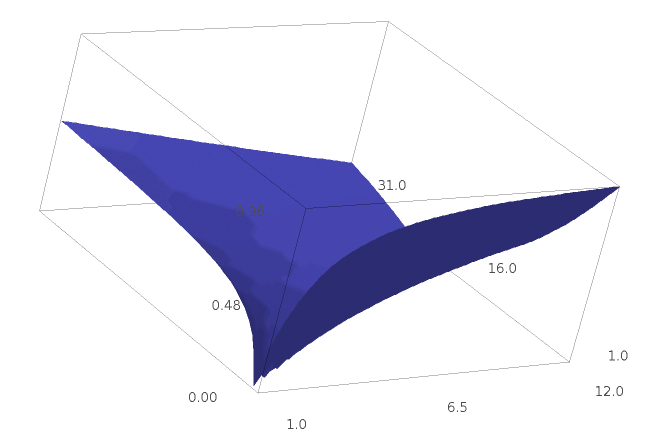
\includegraphics[height=2in]{rcbday.jpg}
          \end{center}
        \item We want to maximize this.
          \begin{equation*}
            \theta
            =
            \arccos(\,\frac{\colvec[r]{7 \\ 12}\dotprod\colvec{m \\ d}}{
                  \norm{\colvec[r]{7 \\ 12}\,}\cdot\norm{\colvec{m \\ d}\,} }\,)
          \end{equation*}
          Of course, we cannot take $m$ or $d$ negative and so we cannot
          get a vector orthogonal to the given one.
          This Python script finds the largest angle by brute force.
          \begin{verbatim}
  import math
  days={1:31,  # Jan
        2:29, 3:31, 4:30, 5:31, 6:30, 7:31, 8:31, 9:30, 10:31, 11:30, 12:31}
  BDAY=(7,12)
  max_res=0
  max_res_date=(-1,-1)
  for month in range(1,13):
      for day in range(1,days[month]+1):
          num=BDAY[0]*month+BDAY[1]*day
          denom=math.sqrt(BDAY[0]**2+BDAY[1]**2)*math.sqrt(month**2+day**2)
          if denom>0:
              res=math.acos(min(num*1.0/denom,1))
              print "day:",str(month),str(day)," angle:",str(res)
              if res>max_res:
                  max_res=res
                  max_res_date=(month,day)
  print "For ",str(BDAY),"the worst case is",str(max_res),"radians on date",str(max_res_date)
  print "  That is ",180*max_res/math.pi,"degrees"
          \end{verbatim}
          The result is 
          \begin{verbatim}
  For  (7, 12) the worst case is 0.95958064648 radians on date (12, 1)
    That is  54.9799211457 degrees
\end{verbatim}

          A more conceptual approach is to consider the relation of all points 
          $(\text{month},\text{day})$ to the point $(7,12)$.
          The picture below
          makes clear that the answer is either Dec~$1$ or Jan~$31$, depending
          on which is further from the birthdate. 
          The dashed line bisects the angle between the line from the
          origin to Dec~$1$, and the line from the origin to Jan~$31$.
          Birthdays above the line are furthest from Dec~$1$ and 
          birthdays below the line are furthest from Jan~$31$.
          \begin{center}
            \includegraphics{ch1.54}
          \end{center}
      \end{exparts}
    \end{answer}
  \puzzle \item 
    \cite{Monthly33p118}
    A ship is sailing with speed and direction \( \vec{v}_1 \); the wind blows
    apparently (judging by the vane on the mast) in the direction of a vector
    \( \vec{a} \); on changing the direction and speed of the ship from
    \( \vec{v}_1 \) to \( \vec{v}_2 \) the apparent wind is in the direction
    of a vector \( \vec{b} \).

    Find the vector velocity of the wind.
    \begin{answer}
      \answerasgiven %
      The actual velocity \( \vec{v} \) of the wind is the sum of the
      ship's velocity and the apparent velocity of the wind.
      Without loss of generality we may assume \( \vec{a} \) and
      \( \vec{b} \) to be unit vectors, and may write
      \begin{equation*}
         \vec{v}=\vec{v}_1+s\vec{a}=\vec{v}_2+t\vec{b}
      \end{equation*}
      where \( s \) and \( t \) are undetermined scalars.
      Take the dot product first by \( \vec{a} \) and then by \( \vec{b} \)
      to obtain
      \begin{align*}
         s-t\vec{a}\dotprod\vec{b}
         &=\vec{a}\dotprod(\vec{v}_2-\vec{v}_1)    \\
         s\vec{a}\dotprod\vec{b}-t
         &=\vec{b}\dotprod(\vec{v}_2-\vec{v}_1)
      \end{align*}
      Multiply the second by \( \vec{a}\dotprod\vec{b} \), 
      subtract the result from the first, and find
      \begin{equation*}
         s=
         \frac{[\vec{a}-(\vec{a}\dotprod\vec{b})\vec{b}]
                   \dotprod(\vec{v}_2-\vec{v}_1)
              }{1-(\vec{a}\dotprod\vec{b})^2}.
      \end{equation*}
      Substituting in the original displayed equation, we get
      \begin{equation*}
         \vec{v}=\vec{v}_1+
         \frac{[\vec{a}-(\vec{a}\dotprod\vec{b})\vec{b}]
                  \dotprod(\vec{v}_2-\vec{v}_1)
              \vec{a}}{1-(\vec{a}\dotprod\vec{b})^2}.
      \end{equation*}  
    \end{answer}
  \item  
     Verify the Cauchy-Schwartz inequality by first proving
     Lagrange's identity:
     \begin{equation*}
      \left(\sum_{1\leq j\leq n} a_jb_j \right)^2
      =
      \left(\sum_{1\leq j\leq n}a_j^2\right)
      \left(\sum_{1\leq j\leq n}b_j^2\right)
      -
      \sum_{1\leq k < j\leq n}(a_kb_j-a_jb_k)^2
     \end{equation*}
     and then noting that the final term is positive.
     (Recall the meaning
     \begin{equation*}
       \sum_{1\leq j\leq n}a_jb_j=
       a_1b_1+a_2b_2+\cdots+a_nb_n
     \end{equation*}
     and
     \begin{equation*}
       \sum_{1\leq j\leq n}{a_j}^2=
       {a_1}^2+{a_2}^2+\cdots+{a_n}^2
     \end{equation*}
     of the \( \Sigma \) notation.)
     This result 
     is an improvement over Cauchy-Schwartz because it gives a formula for
     the difference between the two sides.
     Interpret that difference in \( \Re^2 \).
     \begin{answer}
       We use induction on \( n \).

       In the \( n=1 \) base case the identity reduces to
       \begin{equation*}
          (a_1b_1)^2=({a_1}^2)({b_1}^2)-0
       \end{equation*}
       and clearly holds.

       For the inductive step assume that 
       the formula holds for the \( 0 \), \ldots, \( n \) cases.
       We will show that it then holds in the \( n+1 \) case.
       Start with the right-hand side
       \begin{multline*}
         \bigl( \sum_{1\leq j\leq n+1}{a_j}^2\bigr)
         \bigl( \sum_{1\leq j\leq n+1}{b_j}^2\bigr)
         -
         \sum_{1\leq k<j\leq n+1}\bigl(a_kb_j-a_jb_k\bigr)^2  \\
       \begin{aligned}
         &=
         \bigl[ (\sum_{1\leq j\leq n}{a_j}^2)+{a_{n+1}}^2\bigr]
         \bigl[ (\sum_{1\leq j\leq n}{b_j}^2)+{b_{n+1}}^2\bigr]   \\     
         &\hbox{}\quad -
         \bigl[\sum_{1\leq k<j\leq n}\bigl(a_kb_j-a_jb_k\bigr)^2+
         \sum_{1\leq k\leq n}\bigl(a_kb_{n+1}-a_{n+1}b_k\bigr)^2  \bigr] \\
         &=
         \bigl( \sum_{1\leq j\leq n}{a_j}^2\bigr)
         \bigl( \sum_{1\leq j\leq n}{b_j}^2\bigr)
         +
         \sum_{1\leq j\leq n}{b_j}^2{a_{n+1}}^2                 
         +
         \sum_{1\leq j\leq n}{a_j}^2{b_{n+1}}^2
         +
         {a_{n+1}}^2{b_{n+1}}^2                                 \\
         &\hbox{}\qquad\hbox{} -
         \bigl[\sum_{1\leq k<j\leq n}\bigl(a_kb_j-a_jb_k\bigr)^2+
         \sum_{1\leq k\leq n}\bigl(a_kb_{n+1}-a_{n+1}b_k\bigr)^2  \bigr] \\
         &=
         \bigl( \sum_{1\leq j\leq n}{a_j}^2\bigr)
         \bigl( \sum_{1\leq j\leq n}{b_j}^2\bigr)
         -\sum_{1\leq k<j\leq n}\bigl(a_kb_j-a_jb_k\bigr)^2   \\   
         &\hbox{}\quad +
         \sum_{1\leq j\leq n}{b_j}^2{a_{n+1}}^2
         +
         \sum_{1\leq j\leq n}{a_j}^2{b_{n+1}}^2
         +
         {a_{n+1}}^2{b_{n+1}}^2                                 \\
         &\hbox{}\qquad\hbox{} -
         \sum_{1\leq k\leq n}\bigl(a_kb_{n+1}-a_{n+1}b_k\bigr)^2
        \end{aligned}
       \end{multline*}
       and apply the inductive hypothesis
       \begin{align*}
         &=
         \bigl( \sum_{1\leq j\leq n}a_jb_j\bigr)^2              
         +
         \sum_{1\leq j\leq n}{b_j}^2{a_{n+1}}^2
         +
         \sum_{1\leq j\leq n}{a_j}^2{b_{n+1}}^2
         +
         {a_{n+1}}^2{b_{n+1}}^2                          \\              
         &\hbox{}\qquad\hbox{}-
         \bigl[\sum_{1\leq k\leq n}{a_k}^2{b_{n+1}}^2
           -2\sum_{1\leq k\leq n}a_kb_{n+1}a_{n+1}b_k
           +\sum_{1\leq k\leq n}{a_{n+1}}^2{b_k}^2\bigr]        \\
         &=
         \bigl( \sum_{1\leq j\leq n}a_jb_j\bigr)^2
         +2\bigl(\sum_{1\leq k\leq n}a_kb_{n+1}a_{n+1}b_k\bigr)
         +{a_{n+1}}^2{b_{n+1}}^2                                 \\
         &=
         \bigl[\bigl(\sum_{1\leq j\leq n}a_jb_j\bigr)+a_{n+1}b_{n+1}\bigr]^2
       \end{align*}
       to derive the left-hand side.  
   \end{answer}
\end{exercises}

